\section{Least and greatest element}

We say that $P$ has a $\hat{0}$ if there exists an element $\hat{0} \in P$ such that $t \geq \hat{0}$ for all $t \in P$. Similarly, $P$ has a $\hat{1}$ if there exists $\hat{1} \in P$ such that $t \leq \hat{1}$ for all $t \in P$. We denote by $P$ the poset obtained from $P$ by adjoining a $\hat{0}$ and $\hat{1}$ (in spite of a $\hat{0}$ or $\hat{1}$ that $P$ may already possess). See \ref{fig:stanley:3-3} for an example. \cite{Stanley:2011:ECV:2124415}



\begin{figure}
	\centering
	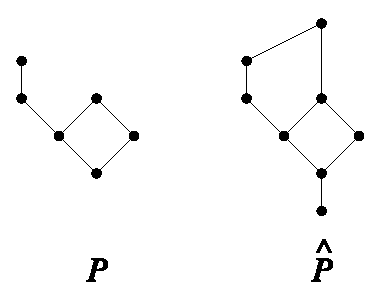
\includegraphics[width=0.5\textwidth]{fig/stanley/3-3}
	\caption{\label{fig:stanley:3-3} Adjoining a $\hat{0}$ and $\hat{1}$. \cite{Stanley:2011:ECV:2124415}}
\end{figure}